\chapter{RESULTS AND DISCUSSION}
{\baselineskip=2\baselineskip
	
This chapter presents the system implementation results and assesses the extent to which the study’s objectives were accomplished. It covers the performance of the detection, tracking, and counting models, the development of the web-based analytics application, and the evaluation of the system’s accuracy and usability within a real-world retail environment.

\section{Implement Computer Vision Models to Detect, Track, and Count Customers using a Multi-camera Approach.}

This section presents the implementation of the SUBAY system’s core computer vision modules for customer detection, tracking, re-identification, counting, and heat mapping. These modules formed the foundation for the system's ability to monitor customer behavior across multiple store zones. The multi-camera pipeline involved detecting customers in each frame, tracking their movements across time, re-identifying them across different camera views, and aggregating these data points for customer analytics.

\subsection{Customer Detection using YOLOv10}

The customer detection module was the initial step in the SUBAY system’s computer vision pipeline. The YOLOv10x model was utilized for this task due to its balance of detection accuracy and real-time performance. According to \cite{Ultralytics2025}, the YOLOv10x model achieved an Average Precision (APval) of 54.4 at an input size of 640×640, with 160.4 GFLOPs and an inference latency of 10.70 milliseconds, confirming its suitability for deployment in the SUBAY system (see Table 4.1).

\begin{table}[htbp]
	\begin{doublespace}
		\centering
		\caption[Performance Metrics for YOLOv10x \citep{Ultralytics2025}]{\newline \newline Performance Metrics for YOLOv10x \citep{Ultralytics2025}}
		\begin{tabular}{|p{3cm}|p{3cm}|p{2.5cm}|p{2.5cm}|p{2.5cm}|}
			\hline
			\textbf{Model} & \textbf{Input Size} & \textbf{AP\(^\text{val}\)} & \textbf{FLOPs (G)} & \textbf{Latency (ms)} \\
			\hline
			YOLOv10x & 640 & 54.4 & 160.4 & 10.70 \\
			\hline
		\end{tabular}
	\end{doublespace}
	\label{tab:yolov10x}
\end{table}

To validate this model’s real-world capacity to detect customers, the researchers conducted a frame-level analysis using pre-recorded video streams from four different camera angles within a retail store. These views captured a range of conditions, including varying crowd densities, lighting environments, and occlusion scenarios. Figure 4.1 displays sample outputs, illustrating the model's ability to localize customers across zones using bounding boxes.

To manage the large volume of video data, Systematic Random Sampling (SRS) was used to extract representative frames from each camera in the test track. The sampling interval $(k)$ was fixed at 30 based on the track’s frame rate, leaving the sample size $(n)$ as the unknown.

\begin{figure}[H]
	\caption[Sample Detection Outputs using YOLOv10x Across Different Camera Angles]{\newline \newline Sample Detection Outputs using YOLOv10x Across Different Camera Angles}
	\centering
	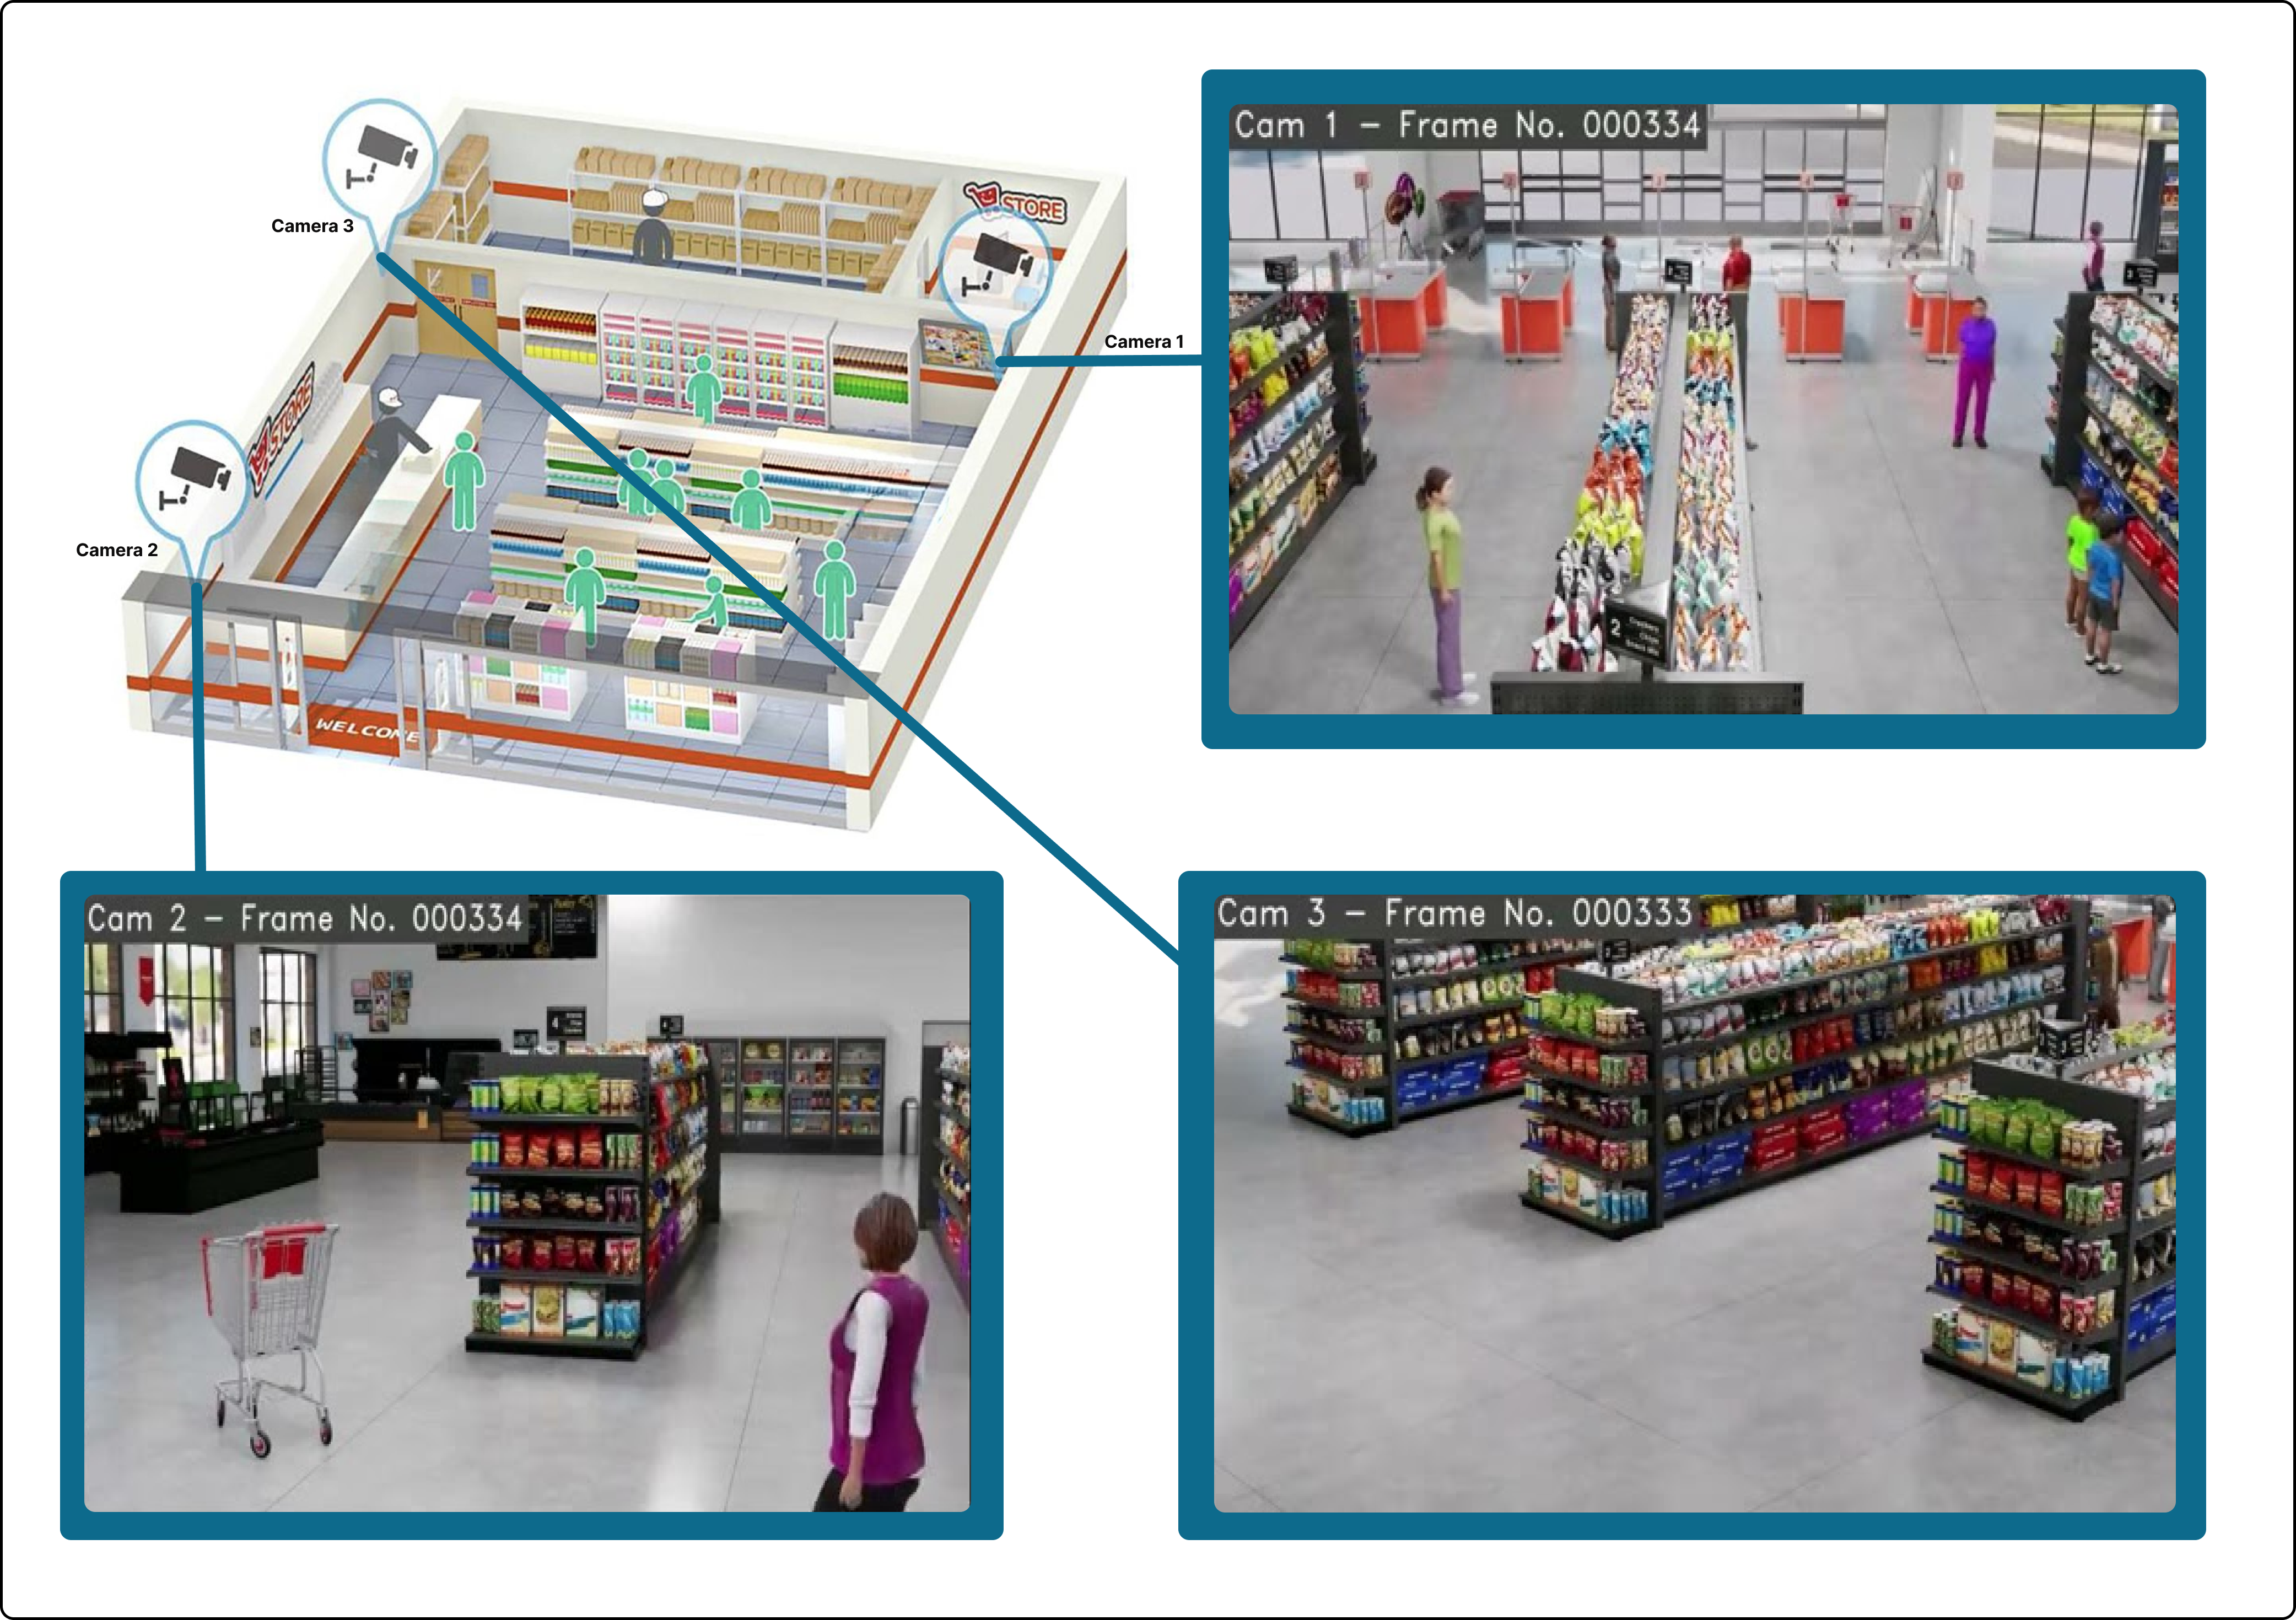
\includegraphics[width=1\linewidth]{fig/4.1}
	\label{fig:4.1}
\end{figure}

Using the SRS formula, the total number of frames $(N = 13, 888)$ was divided by $k$ ($k$ = number of frames per second of the video) to obtain $n = 463$ frames. Table 4.2 presents the detailed calculations of sampled frames per camera based on this method. Table 4.2 presents the detailed calculations of sampled frames per camera based on this method.


{\doublespacing
	\begin{longtable}{|p{4cm}|p{5cm}|p{5cm}|}
		\caption[Sampling Methodology Overview]{\newline \newline Sampling Methodology Overview} \label{tab:sampling} \\
		\hline
		\textbf{Camera} & \textbf{Total Frames} & \textbf{Sampled Frames} \\
		\hline
		\endfirsthead
		
		\multicolumn{3}{l}{\tablename\ \thetable{} -- \textit{continued from previous page}} \\
		\hline
		\textbf{Camera} & \textbf{Total Frames} & \textbf{Sampled Frames} \\
		\hline
		\endhead
		
		\hline \multicolumn{3}{|r|}{\textit{Continued on next page}} \\ \hline
		\endfoot
		
		\hline
		\endlastfoot
		
		Camera 1 & 3,301 & 110 \\
		\hline
		Camera 2 & 4,199 & 140 \\
		\hline
		Camera 3 & 2,189 & 73 \\
		\hline
		Camera 4 & 4,199 & 140 \\
		\hline
		\textbf{Total} & \textbf{13,888} & \textbf{463} \\
		\hline
		
	\end{longtable}
}


Each sampled frame was then manually annotated to record the following metrics:

\noindent
\begin{itemize}
	\item $\text{True Positives (TP)}$ - correctly detected customers
	\item $\text{False Positives (FP)}$ - non-customers incorrectly identified as customers
	\item $\text{False Negatives (FN)}$ - missed customer detections
	\item $\text{True Negatives (TN)}$ - correctly undetected non-customers (not directly countable)
\end{itemize}

Based on this annotation, the Precision, Recall, and F1 Score were calculated for each camera to assess the model’s performance in practical store conditions (see Table 4.3).

Across all cameras, the model yielded 100\% precision, indicating no false positives after refinement. However, recall values ranged from 89.15\% to 93.06\%, reflecting some missed detections due to occlusion or distance from the camera.

\begin{table}[H]
	\begin{doublespace}
		\centering
		\caption[YOLOv10x Model Accuracy based on the Elements of a Confusion Matrix]{\newline \newline YOLOv10x Model Accuracy based on the Elements of a Confusion Matrix}
		\resizebox{\textwidth}{!}{%
			\begin{tabular}{|p{1.9cm}|p{2.1cm}|p{2.1cm}|p{2.1cm}|p{1.7cm}|p{1.7cm}|p{1.7cm}|p{1.7cm}|}
				\hline
				\textbf{Camera} & \textbf{Total True Positives} & \textbf{Total False Positives} & \textbf{Total False Negatives} & \textbf{Total True Negatives} & \textbf{Precision} & \textbf{Recall} & \textbf{F1 Score}\\
				\hline
				Camera 1 & 411 & 0 & 50 & 20 & 100.00\% & 89.15\% & 94.27\% \\
				\hline
				Camera 2 & 582 & 0 & 61 & 8 & 100.00\% & 90.51\% & 95.02\% \\
				\hline
				Camera 3 & 440 & 0 & 50 & 0 & 100.00\% & 89.80\% & 94.62\% \\
				\hline
				Camera 4 & 738 & 0 & 55 & 0 & 100.00\% & 93.06\% & 96.41\% \\
				\hline
				\textbf{SUM} & \textbf{2171} & \textbf{0} & \textbf{216} & \textbf{28} & \textbf{100.00\%} & \textbf{90.95\%} & \textbf{95.26\%} \\
				\hline
				\textbf{AVERAGE} & \textbf{542.75} & \textbf{0} & \textbf{54} & \textbf{7} & \textbf{100.00\%} & \textbf{90.95\%} & \textbf{95.26\%} \\
				\hline
			\end{tabular}
		}
	\end{doublespace}
\end{table}

Per-camera observations revealed unique detection challenges. Camera 1 experienced detection inconsistencies due to the people visible at the frame’s edge and occasional occlusions caused by shelves or customers entering/exiting the view. Camera 2 was positioned above a densely populated checkout area. Heavy foot traffic, edge-of-frame individuals, and partial occlusion contributed to the model missing some customers. Camera 3 had an ideal angle, avoiding cashier zones and outside interference. It maintained high precision and recall even in slightly occluded scenarios. Camera 4 delivered the most optimal performance. Despite crowd density, it consistently detected customers while lighting conditions were stable.

\begin{figure}[H]
	\caption[YOLOv10 F1 Curve]{\newline \newline YOLOv10 F1 Curve}
	\centering
	\includegraphics[width=0.70\linewidth]{fig/4.2.pdf}
	\label{fig:4.2}
\end{figure}

For the model training and fine-tuning, a dataset comprising 10,635 images of people was integrated into an existing pre-trained model to train a people detection model further using YOLOv10. As shown in the figure, the trained model attained an F1 score of 0.88 at a confidence threshold of 0.80 for the "person" class. This performance suggests that the model effectively detects individuals in videos with high precision and recall at the specified confidence level.

\subsection{Customer Tracking using DeepSORT}

After detecting customers, the system used the DeepSORT algorithm to assign and maintain unique tracking IDs across consecutive video frames and overlapping store zones. While effective in many scenarios, DeepSORT faced difficulty maintaining consistent IDs across all four cameras. ID switches occurred during transitions between views, in poor lighting conditions, or when individuals were partially obscured. These issues were more common near frame edges or in crowded areas. However, DeepSORT often re-identified individuals after temporary disappearance, particularly when they returned to the center of the frame. Figure~\ref{fig:4.3} shows a sample frame with consistent and inconsistent ID assignments during tracking.

\begin{figure}[H]
	\caption[Consistent and Inconsistent ID Assignments during DeepSORT Tracking]{\newline \newline Consistent and Inconsistent ID Assignments during DeepSORT Tracking}	
	\centering
	\includegraphics[width=1\linewidth]{fig/4.3.pdf}
	\label{fig:4.3}
\end{figure}

To evaluate DeepSORT's performance, a set of designated video test clips was extracted from various in-store conditions. Table 4.4 summarizes the tracking outcomes using key performance indicators:

\textit{- Total Tracked Customers} refers to the number of unique individuals detected and monitored throughout a test sequence.

\textit{- ID Switches} capture instances where DeepSORT mistakenly assigned a different ID to the same person, indicating a lapse in identity preservation.

\textit{- Re-ID Success Rate (\%)} measures the algorithm's ability to successfully re-identify individuals after temporary occlusion or after exiting and re-entering a frame. It is calculated as:

\begin{equation}
	\text{Re-ID Success Rate} = (\frac{\textit{Total Tracked Customers - ID Switches}}{\textit{Total Tracked Customers}}) \times 100
\end{equation}
\myequation{Re-ID Success Rate}

This metric conceptually aligns with the Rank-1 Accuracy used in person re-identification benchmarks, where a correct match is counted if the correct identity appears as the top-ranked result \citep{Zheng2015}. While simplified, this formulation remains effective for evaluating practical system-level performance in real-world environments.

The performance results of DeepSORT across the different in-store scenarios highlighted its strengths and limitations. The algorithm successfully tracked many customers in regular traffic aisles, but 45 ID switches led to a moderate Re-ID success rate of 53\%.

\begin{table}[H]
	\centering
	\caption[Customer Tracking Performance Across Different Retail Scenarios]{\newline \newline Customer Tracking Performance Across Different Retail Scenarios}
	\begin{tabular}{|p{1.5cm}|p{1.5cm}|p{1.5cm}|p{1.8cm}|p{3.5cm}|}
		\hline
		\textbf{Scenario} & \textbf{Total Tracked Customers} & \textbf{ID Switches} & \textbf{Re-ID Success Rate (\%)} & \textbf{Notes:} \\
		\hline
		Normal traffic aisle & 96 & 45 & 53\% & Moderate foot traffic with occasional occlusion \\
		\hline
		Crowded aisle & 32 & 17 & 47\% & High density, overlapping paths, and frame-edge exits \\
		\hline
		Occlusion-heavy zones & 24 & 18 & 25\% & Frequent obstruction by shelves, other customers, or fixtures \\
		\hline
		Camera transition zones & 21 & 11 & 48\% & Movement across overlapping fields of view and lighting changes \\
		\hline
	\end{tabular}
	\label{tab:customer_tracking}
\end{table}

Performance declined in crowded aisles and occlusion-heavy zones, where overlapping paths and frequent obstructions caused more ID mismatches, resulting in lower Re-ID rates of 47\% and 25\%, respectively. The camera transition zones posed additional challenges due to changes in angles and lighting, achieving a Re-ID success rate of 48\%. These results indicate that while DeepSORT can work in less complex conditions, its identity consistency degrades in visually dynamic or cluttered environments, an essential consideration for improving system robustness.

\subsection{Re-Identification with Omni-Scale Network}

To address DeepSORT’s limitations in maintaining consistent identity tracking across multiple overlapping camera frames, the system incorporated a Person Re-Identification (Re-ID) model. This model aimed to enhance cross-view identity continuity by re-matching customers based on visual features, even when tracked IDs were disrupted due to occlusion, crowding, or camera transitions.

The Re-ID model was trained using annotated image datasets containing customer appearances across multiple store cameras. Feature embeddings were extracted and processed using the Omni-Scale Network (OSNet), a deep learning architecture known for its robust performance in cross-view appearance matching as discussed in the previous chapter.

\begin{figure}[H]
	\caption[Sample Customers in the Re-identification Dataset Across Different Camera Views]{\newline \newline Sample Customers in the Re-identification Dataset Across Different Camera Views}
	\centering
	\includegraphics[width=0.75\linewidth]{fig/4.4.pdf}
	\label{fig:4.4}
\end{figure}

Figure~\ref{fig:4.4} presents sample subjects from the training dataset, arranged in camera sequence from left to right: Camera 02, Camera 05, Camera 03, and Camera 09.

After training, the model was evaluated using a test dataset, achieving an accuracy of 75.48\%, a precision of 73.70\%, a recall of 70.70\%, and an F1-score of 72.17\% as summarized in Table 4.5. These metrics confirmed the model’s reliability in controlled testing environments, validating its integration into the multi-camera tracking pipeline for retail analytics.

\begin{table}[htbp]
	\begin{doublespace}
		\centering
		\caption[Re-Identification Model Training Results]{\newline \newline Re-Identification Model Training Results}
		\begin{tabular}{|c|c|c|c|}
			\hline
			\textbf{Accuracy} & \textbf{Precision} & \textbf{Recall} & \textbf{F1-Score} \\
			\hline
			75.48 & 73.70 & 70.70 & 72.17 \\
			\hline
		\end{tabular}
	\end{doublespace}
\end{table}

The trained Re-ID model was tested on a video sequence featuring customer movements across overlapping store zones to assess its applicability in real-world conditions. The aim was to evaluate how the model responded to typical challenges such as occlusions, dynamic lighting, and varying subject positions.

Figure~\ref{fig:4.5} shows Case A, in which the same individual was correctly identified across all four camera views. This ideal scenario occurred under good lighting and centered framing, confirming optimal model behavior.

\begin{figure}[H]
	\caption[Re-Identification Case A: Perfect Re-Identification Across All Camera Views]{\newline \newline Re-Identification Case A: Perfect Re-Identification Across All Camera Views}
	\centering
	\includegraphics[width=1\linewidth]{fig/4.5.pdf}
	\label{fig:4.5}
\end{figure}

Figure~\ref{fig:4.6} presents Case B, a near-complete match disrupted by heavy shelf occlusion in the fourth view. The subject was successfully re-identified in the first three views but was missed in the obstructed one.

\begin{figure}[H]
	\caption[Re-Identification Case B: Near-complete Re-Identification Affected by Shelf Occlusion]{\newline \newline Re-Identification Case B: Near-complete Re-Identification Affected by Shelf Occlusion}
	\centering
	\includegraphics[width=0.75\linewidth]{fig/4.6.pdf}
	\label{fig:4.6}
\end{figure}

Case C (Figure~\ref{fig:4.7}) represented a more difficult scenario. The model correctly re-identified the subject in only two of the four views. The remaining views experienced ID switches due to occlusion, off-angle appearances, and varied lighting conditions commonly encountered in operational environments.

While OSNet significantly enhanced identity retention across overlapping camera views, its effectiveness was influenced by external factors. The system performed well in clear, centered, and well-lit frames, but struggled with occlusion, off-angle shots, and inconsistent illumination. These findings underscore the need for improved scene normalization techniques or camera placements that reduce ambiguity in customer visibility.

\begin{figure}[H]
	\caption[Re-Identification Case C: Partial Re-Identification with ID Switches in Overlapping Views]{\newline \newline Re-Identification Case C: Partial Re-Identification with ID Switches in Overlapping Views}
	\centering
	\includegraphics[width=1\linewidth]{fig/4.7.pdf}
	\label{fig:4.7}
\end{figure}

Despite these limitations, the OSNet-based Re-ID model played a critical role in bridging the identity gaps that DeepSORT alone could not resolve, ultimately strengthening the accuracy of the system's behavioral analytics in complex retail environments.

\subsection{Customer Counting Mechanisms}
The customer counting module combined YOLOv10, DeepSORT, and tripline analysis to estimate customer entries and monitor presence across designated store zones. Upon booting the system, the customers it “sees” were assigned unique tracking IDs. An ROI tripline is also virtually placed at the store entrance on one camera frame. This approach prevented double-counting by ensuring each individual was only counted once per entry event. Figure~\ref{fig:4.8} presents a sample frame showing the total customer count and the current count in the store.

\begin{figure}[H]
	\caption[Sample Frame Showing Total Customer Count and Current Count in the Store]{\newline \newline Sample Frame Showing Total Customer Count and Current Count in the Store}
	\centering
	\includegraphics[width=0.75\linewidth]{fig/4.8.pdf}
	\label{fig:4.8}
\end{figure}

Once detected and assigned a unique ID, the system continuously monitored the customer’s movement and logged their presence duration. This enabled the calculation of individual dwell time and overall customer traffic within the monitored space. A summary of results from a test track is provided in Table 4.6.

Total Foot Traffic refers to the number of unique individuals detected by the system, assigned a unique ID, and successfully tracked during the test period. Total Customer Dwell Time represented the cumulative duration, in both seconds and minutes, that all tracked customers spent in the store zone. Average Dwell Time was computed by dividing the total dwell time by the total foot traffic, indicating how long a typical customer remained in the observed area.

\begin{table}[H]
	\begin{doublespace}
		\centering
		\caption[Summary of Customer Count and Dwell Time Based on Test Track]{\newline \newline Summary of Customer Count and Dwell Time Based on Test Track}
		\resizebox{\textwidth}{!}{%
			\begin{tabular}{|p{2.5cm}|p{2.5cm}|p{2.5cm}|p{2.5cm}|p{2cm}|p{2cm}|p{2cm}|}
				\hline
				\textbf{Total Foot Traffic} & \textbf{Total Customer Dwell Time (secs)} & \textbf{Total Customer Dwell Time (min)} & \textbf{Average Dwell Time (secs)} & \textbf{Average Dwell Time (mins)} \\
				\hline
				33 & 4,877.17 & 81.29 & 147.79 & 2.46 \\
				\hline
			\end{tabular}
		}
	\end{doublespace}
\end{table}

These results demonstrated the system’s ability to accurately count foot traffic and analyze customer engagement time. Such data can inform critical operational decisions, including staff allocation, store layout adjustments, and targeted marketing efforts. The ability to measure both frequency and duration of customer visits provided actionable insights for enhancing in-store experiences and improving overall retail performance.

\subsection{Zone-Based Analytics and Heat Map Visualization}

The system implemented zone-based counting and heat map visualization to generate deeper insights into customer movements and behavior. Key store areas, such as aisles and product displays, were designated as Regions of Interest (ROIs) to monitor and quantify customer presence and movement. Aggregated movement data across these zones enabled the generation of heat maps that visually represented both dwell time and customer density. Figure~\ref{fig:4.9} shows a sample heat map overlay that visualizes the intensity of customer activity.

Figure~\ref{fig:4.9} presents a visual overlay combining camera footage with a dynamic heatmap. This visualization serves as an analytical tool to monitor customer movement, density, and dwell time within distinct product zones of the store. Each aisle holds different kinds of products like Aisle 1 with Body and Bath Products, Aisle 2 with Face and Hair Care Products, Aisle 3 with Cosmetics, Aisle 4 with Assorted Home Essentials, Aisle 5 with Kitchenwares, and Aisle 6 with Home Products. Warmer areas on the heatmap indicate zones with heavier foot traffic or longer dwell time, while cooler areas suggest less interaction. This allows store managers to assess which product categories attract more attention, optimize layout design, and make data-driven decisions on product placement or promotions.

\begin{figure}[H]
	\caption[Heatmap Overlay Indicating Customer Density and Dwell Time]{\newline \newline Heatmap Overlay Indicating Customer Density and Dwell Time}
	\centering
	\includegraphics[width=0.75\linewidth]{fig/4.9.pdf}
	\label{fig:4.9}
\end{figure}

\subsection{Accuracy of System-Generated Tracking Compared to Manual Observation}

To evaluate the effectiveness of the SUBAY system in detecting and tracking customers within a retail environment, a comparative analysis was performed between manual annotations and system-generated outputs. This assessment aimed to determine how closely the system could replicate the accuracy of human observation when identifying customer locations over time.

\begin{figure}[H]
	\caption[Intersection over Union (IoU) per Frame]{\newline \newline Intersection over Union (IoU) per Frame}
	\centering
	\includegraphics[width=0.85\linewidth]{fig/4.10.pdf}
	\label{fig:4.10}
\end{figure}

Figure~\ref{fig:4.10} shows two line graphs that illustrate this comparison using data collected from over 5,000 frames of synchronized video footage. The first graph at the top displays the level of overlap between the bounding boxes drawn manually (ground truth) and those generated by the system. This overlap is expressed as a value between 0 and 1, where 1 represents perfect alignment. The graph shows that the overlap remained consistently high throughout the frames, with most values hovering around 0.9 or above. The average overlap achieved was approximately 0.9190, suggesting that the system was highly accurate in placing detection boxes around customers nearly the same way a human would.

\begin{figure}[H]
	\caption[Center Distance per Frame]{\newline \newline Center Distance per Frame}
	\centering
	\includegraphics[width=0.85\linewidth]{fig/4.11.pdf}
	\label{fig:4.11}
\end{figure}

Figure~\ref{fig:4.11} illustrates the distance, measured in pixels, between the centers of the manually and system-drawn boxes for each frame. Lower values in this graph represent closer agreement between the two. The average distance recorded was 6.71 pixels, which is considered minimal and indicates that even when there were slight differences in the size or shape of the boxes, the system still correctly pinpointed the customer's general location.

These two visualizations demonstrate that the SUBAY system could precisely track customer movement across frames. The consistently high overlap and low center distance highlight the reliability of the system’s detection accuracy, closely matching manual observation. This level of performance is crucial for ensuring the validity of customer behavior analytics derived from system-tracked data, such as counting foot traffic, analyzing dwell time, and generating heat maps. The close agreement between manual and automated tracking further supports the system’s readiness for deployment in real-world retail settings where accurate customer insights are essential.

\subsection{Evaluation of Multi-Object Tracking Accuracy and Performance Metrics}

A performance analysis was conducted to evaluate the object tracking capabilities of the SUBAY system using a unified tracking configuration. This setup employed YOLOv10 integrated with DeepSORT and enhanced by the Omni-Scale Re-Identification (Re-ID) module. The system’s effectiveness is visualized using widely accepted multi-object tracking evaluation indicators, as outlined by the studies of \cite{Amosa2023}, \cite{Fei2023}, and \cite{Li2023}. These metrics include: Multiple Object Tracking Accuracy (MOTA), Multiple Object Tracking Precision (MOTP), Identification Precision (IDP), Identification Recall (IDR), and the Identification F1 Score (IDF1).

\begin{figure}[H]
	\caption[Performance of the YOLOv10 + DeepSORT + Omni-Scale Re-ID System]{\newline \newline Performance of the YOLOv10 + DeepSORT + Omni-Scale Re-ID System}
	\centering
	\includegraphics[width=0.85\linewidth]{fig/4.12.pdf}
	\label{fig:4.12}
\end{figure}

Figure~\ref{fig:4.12} presented in this subsection, illustrates the performance of the YOLOv10 + DeepSORT + Omni-Scale Re-ID system across five key multi-object tracking evaluation metrics: MOTA, MOTP, IDP, IDR, and IDF1. Each score is displayed as a point along the vertical axis, ranging from 0 to 1, where higher values indicate better performance.

Starting with MOTA (Multiple Object Tracking Accuracy), the system achieves a score of 0.602, indicating solid overall tracking performance. This metric encapsulates false positives, false negatives, and identity switches. Hence, a score above 0.6 demonstrates the system's capability to track multiple individuals with reasonable consistency, especially in complex, real-world environments involving multiple cameras, occlusions, and identity changes.

The MOTP (Multiple Object Tracking Precision) is notably high at 0.910, showcasing the system’s ability to localize targets accurately within each frame. This score reflects the spatial precision of bounding boxes, suggesting that YOLOv10 detections are tightly aligned with ground-truth person locations. This is crucial for precise and reliable visualization in surveillance or retail analytics.

For Identification Precision (IDP), the system records a score of 0.577, reflecting the proportion of correctly assigned identities among all identity predictions. While this value is moderate, it underscores the inherent complexity of re-identification in a multi-camera system, especially one involving four camera views. IDP is only rewarded in this setup when the same individual is consistently recognized across all four camera streams within the same frame instance (see figure~\ref{fig:4.5}). This constraint introduces evaluation challenges: if the system requires several frames to accumulate enough visual information to match a person across views confidently, say, identifying a person correctly only by the fourth frame, then the earlier mismatches reduce the precision score. In this instance, a correct identification occurring only once across four frames would contribute just 25\% (1/4) to the IDP metric, even if the system eventually makes the right call. As a result, the IDP score may underrepresent the system’s true long-term identity tracking capability, especially when appearance changes, occlusions, or view transitions delay accurate matching across all camera views.

However, in Identification Recall (IDR), a measure of how many true identities were correctly retrieved, the system is slightly higher at 0.612, meaning it is relatively better at retrieving the correct identities among the ground-truth individuals. This implies that the Re-ID module, based on Omni-Scale feature extraction, effectively matches many individuals across camera views, even if not all identity assignments are precise.

Finally, the IDF1 score, which combines a balanced harmonic mean of IDP and IDR, resulted in 0.595, highlighting the system’s overall identity tracking performance. This value reflects a reasonable balance between correct identity assignment and retrieval. It also demonstrates the Re-ID model’s ability to preserve identity over time and across camera views with moderate success.

These results highlight the effectiveness of combining Omni-Scale Re-ID with YOLOv10 + DeepSORT for multi-camera person tracking. The notably high MOTP underscores the system’s strong detection accuracy, while the MOTA and IDF1 scores indicate reliable tracking performance and identity consistency even in complex, multi-view environments. Despite some limitations in identity precision, particularly in early cross-camera associations, the system demonstrates considerable potential for real-world deployments, especially in domains like retail analytics, intelligent surveillance, and multi-camera monitoring, where sustained identity tracking across diverse scenes is essential.

\section{Develop a Web Application for Data Visualization and Customer Analytics from the Results of the Detection, Tracking, and Customer Counting Models.}

A responsive and user-friendly web application was then developed to serve as the main platform for presenting the outputs of the detection, tracking, and customer counting models. Using Firebase for backend support, the system provided real-time updates and organized the visualized data through interactive dashboards and charts. Each page of the application was structured to help users interpret customer behavior more effectively, with features ranging from secure login and live analytics to post-event analysis and insight generation.

\subsection{User Access and Navigation Structure}

The web application consisted of several core pages and functionalities. Upon launching the system, users were greeted with the Welcome Page. As shown in Figure~\ref{fig:4.13}, the Welcome Page featured the (1) SUBAY Logo positioned prominently at the center to establish branding, the (2) Thesis Title displayed adjacent to it to introduce the project, and the (3) Login Button located beneath the title, allowing users to proceed to the secure login page.

\begin{figure}[H]
	\caption[Welcome Page]{\newline \newline Welcome Page}
	\centering
	\includegraphics[width=1\linewidth]{fig/4.13.pdf}
	\label{fig:4.13}
\end{figure}

The system then directed users to the Login Page. Figure~\ref{fig:4.14} depicts the Login Page layout, which included several critical functional elements: the (1) Log in Box where all credentials were entered, the (2) Log in Title positioned at the top to guide users, the (3) Email Credential input field, and the (4) Password Credential input field essential for authentication. Below the input fields, the (5) Log in Button was provided to initiate the login process, and below the form, the (6) Copyright Statement acknowledged the work's intellectual property.

\begin{figure}[H]
	\caption[Login Page]{\newline \newline Login Page}
	\centering
	\includegraphics[width=1\linewidth]{fig/4.14.pdf}
	\label{fig:4.14}
\end{figure}

After successful authentication, users were redirected to the Dashboard Page, which served as the central hub of the SUBAY system. As shown in Figure 4.15, the dashboard offered streamlined access to all major features and presented a comprehensive overview of system insights. On the left side, the (1) Sidebar Menu provided navigational access to key modules such as the (3) Home Page, (4) Live Analytics Page, (5) Heatmapping Page, (6) Post Analytics Page, (7) Insights Page, and (8) About Page. Users could also minimize the sidebar using the (2) Collapse Sidebar Button to maximize screen space.

\begin{figure}[H]
	\caption[Dashboard Page]{\newline \newline Dashboard Page}
	\centering
	\includegraphics[width=1\linewidth]{fig/4.15.pdf}
	\label{fig:4.15}
\end{figure}

At the top of the interface, the (9) Topbar / Title indicated the current section being viewed, while the (10) User Toggle Button allowed access to account settings and logout functionality. Within the main dashboard view, direct navigation was provided through quick-access buttons, including the (11) Direct Route to Live Analytics Page, (12) Heatmapping Page, (13) Post Analysis Page, and (14) Insights Page.

The dashboard also displayed a variety of interactive components. The (15) Camera Feed Card previewed video input from active feeds, while the (17) Live Cameras Available Card and (18) Available Dates Card helped users identify currently active cameras and available analytics data. Visual summaries were presented through the (22) Total Foot Traffic Pie Chart, (24) Average Dwell Time Line Chart, and (25) Aisle-Based Foot Traffic and Dwell Time Bar Chart, providing clear overviews of behavioral patterns.

To highlight key insights at a glance, the dashboard featured the (19) Peak Visit Aisle Card and (20) Peak Dwell Aisle Card, showing which zones had the highest foot traffic and longest dwell time, respectively. The (21) Live Analysis Card displayed dynamic tracking metrics. Users could also access deeper analysis via the (16) Open Live Analytics Page and the (23) Open to Insights Page options. Finally, a (26) Theme Toggle allowed users to switch between dark and light modes for a more personalized viewing experience.

\subsection{Real-time Analysis}

\begin{figure}[H]
	\caption[Live Analytics Page]{\newline \newline Live Analytics Page}
	\centering
	\includegraphics[width=0.80\linewidth]{fig/4.16.pdf}
	\label{fig:4.16}
\end{figure}

The Live Analytics Page, displayed in Figure~\ref{fig:4.16}, demonstrated real-time monitoring capabilities of the system. The page consisted of several key components: the (1) Live Analytics Feed, presenting a real-time view of detected customers, the (2) Live Total Customer Count summarizing the cumulative foot traffic, the (3) Live Current Customers Count showing the active number of customers within the store, the (4) Live Total Aisle Visits tracking customer movement across zones, and the (5) Live Average Dwell Time (in seconds) providing immediate insight into customer engagement duration.

\begin{figure}[H]
	\caption[Heat Mapping Page]{\newline \newline Heat Mapping Page}
	\centering
	\includegraphics[width=1\linewidth]{fig/4.17.pdf}
	\label{fig:4.17}
\end{figure}

The system also featured a Heat Mapping Page for spatial behavior visualization. As shown in Figure~\ref{fig:4.17}, the Heat Mapping Page consisted of the (1) Camera Feed displaying the active surveillance view and the (2) Heat map Overlay applied atop the feed, illustrating customer density and movement patterns with color gradients.

\subsection{Post-Event Analysis}

\begin{figure}[H]
	\caption[Post Analytics Page]{\newline \newline Post Analytics Page}
	\centering
	\includegraphics[width=1\linewidth]{fig/4.18.pdf}
	\label{fig:4.18}
\end{figure}

The Post Analytics Page enables users to analyze store performance after events. Figure 4.18 shows the Post Analytics Page, which incorporated the following elements: (1) Customer and Zone-based Counting to contrast movement trends, (2) Heat Map Overlay for post-event spatial distribution, (3) Total Foot Traffic metrics, (4) Average Dwell Time measurements, and (5) Aisle-Based Foot Traffic and Dwell Time distributions, providing actionable insights on customer interactions with different store zones.

\begin{figure}[H]
	\caption[Insights Page]{\newline \newline Insights Page}
	\centering
	\includegraphics[width=1\linewidth]{fig/4.19.pdf}
	\label{fig:4.19}
\end{figure}

As presented in Figure~\ref{fig:4.19}, the Insights Page consolidated analytical findings into strategic recommendations. Functional elements included the peak metrics cards, (1) Aisle with the highest visit indicator, and (2) Aisle with the highest dwell time indicator to highlight critical engagement areas. Three charts were provided with user interaction options: the (3) Total Foot Traffic Pie Chart with an integrated Date Range Picker and Expand Button, the (4) Average Dwell Time per Aisle Line Chart with similar interactive controls, and the (5) Aisle-Based Foot Traffic and Dwell Time Bar Chart. Additionally, the (6) Generate Insights Button was incorporated to automate the generation of narrative summaries based on the analyzed data.

\subsection{Insight Generation}
One of the significant outcomes of the system's development was the integration of an automated insight generation module, as outlined in the Activity Diagram for Insight Generation. This module processed the aggregated outputs from customer detection, tracking, and counting to derive high-level behavioral analytics. Through this workflow, the system transformed raw customer movement data into concise summaries, logical conclusions, and actionable recommendations designed to support informed decision-making by store managers.

\begin{figure}[H]
	\caption[Insight Generation]{\newline \newline Insight Generation}
	\centering
	\includegraphics[width=0.8\linewidth]{fig/4.20.pdf}
	\label{fig:4.20}
\end{figure}

The Insight Generation functionality was accessed through the Insights Page of the web application, as shown in Figure~\ref{fig:4.20}. The system automatically computed several key performance metrics after collecting detection and tracking outputs over a monitoring period. These included:

\noindent - Total Foot Traffic: The number of unique entries during the monitored period.

\noindent - Peak Day Analysis: Identifying the day with the most customer entries.

\noindent - Zone-Based Foot Traffic: Highlighting which aisle attracted the most traffic.

\noindent - Zone-Based Dwell Time: Measuring where customers lingered the longest.

\noindent - Average Dwell Time: Calculated across all store zones to gauge overall engagement.

\begin{figure}[H]
	\caption[Sample Generated Analytics Report Output]{\newline \newline Sample Generated Analytics Report Output}
	\centering
	\includegraphics[width=1\linewidth]{fig/4.21.pdf}
	\label{fig:4.21}
\end{figure}

Figure~\ref{fig:4.21} presents the sample downloadable generated analytics report output. These computations were processed programmatically through the web application's backend, where pieChartData and barChartData were analyzed to derive summarized figures. Specific computations included summing total entries, calculating total traffic per zone percentages, identifying top-performing and underperforming aisles, and determining average and peak dwell times.

These values were then evaluated against industry performance thresholds. According to BPlanAI (2025) and \cite{CountTrack2025}, retail stores with beauty items typically see 50–80 daily visitors, and healthy customer dwell time ranges between 10 and 20 minutes. Using this guidance, the system programmatically flagged the store as performing well since:

\noindent - The Average Daily Foot Traffic was 51.80, well above the minimum benchmark.

\noindent - Average Customer Dwell Time was 11.31 minutes, indicating sustained engagement.

The results were automatically compiled into a downloadable Retail Insight Report, which presented the findings in a user-friendly format, such as in the sample report shown in Figure 4.22.

\noindent - The total foot traffic recorded during the monitoring period was 259 entries.

\noindent - The peak day was April 13, 2025, with 78 entries (30.12\% of all traffic).

\noindent - Aisle B emerged as the zone with the highest foot traffic, accounting for 30 recorded entries (39.38\%).

\noindent - Aisle A was highlighted as the zone with the longest total dwell time, totaling 105.38 minutes.

\noindent - The total customer dwell time across all zones is 339.3 minutes, and the average dwell time across all zones is 11.31 minutes, indicating a healthy level of customer engagement.

Beyond numerical reporting, the system generated conclusions based on pre-established logic conditions.

\begin{figure}[H]
	\caption[Sample Report’s Results]{\newline \newline Sample Report’s Results}
	\centering
	\includegraphics[width=1\linewidth]{fig/4.22.pdf}
	\label{fig:4.22}
\end{figure}

In Figure~\ref{fig:4.23}, the system concluded, "The store is performing well, recording an average of 51.80 daily foot traffic with an average dwell time of 11.31 minutes.” This indicates healthy foot traffic and meaningful customer engagement.

\begin{figure}[H]
	\caption[Sample Report’s Conclusions]{\newline \newline Sample Report’s Conclusions}
	\centering
	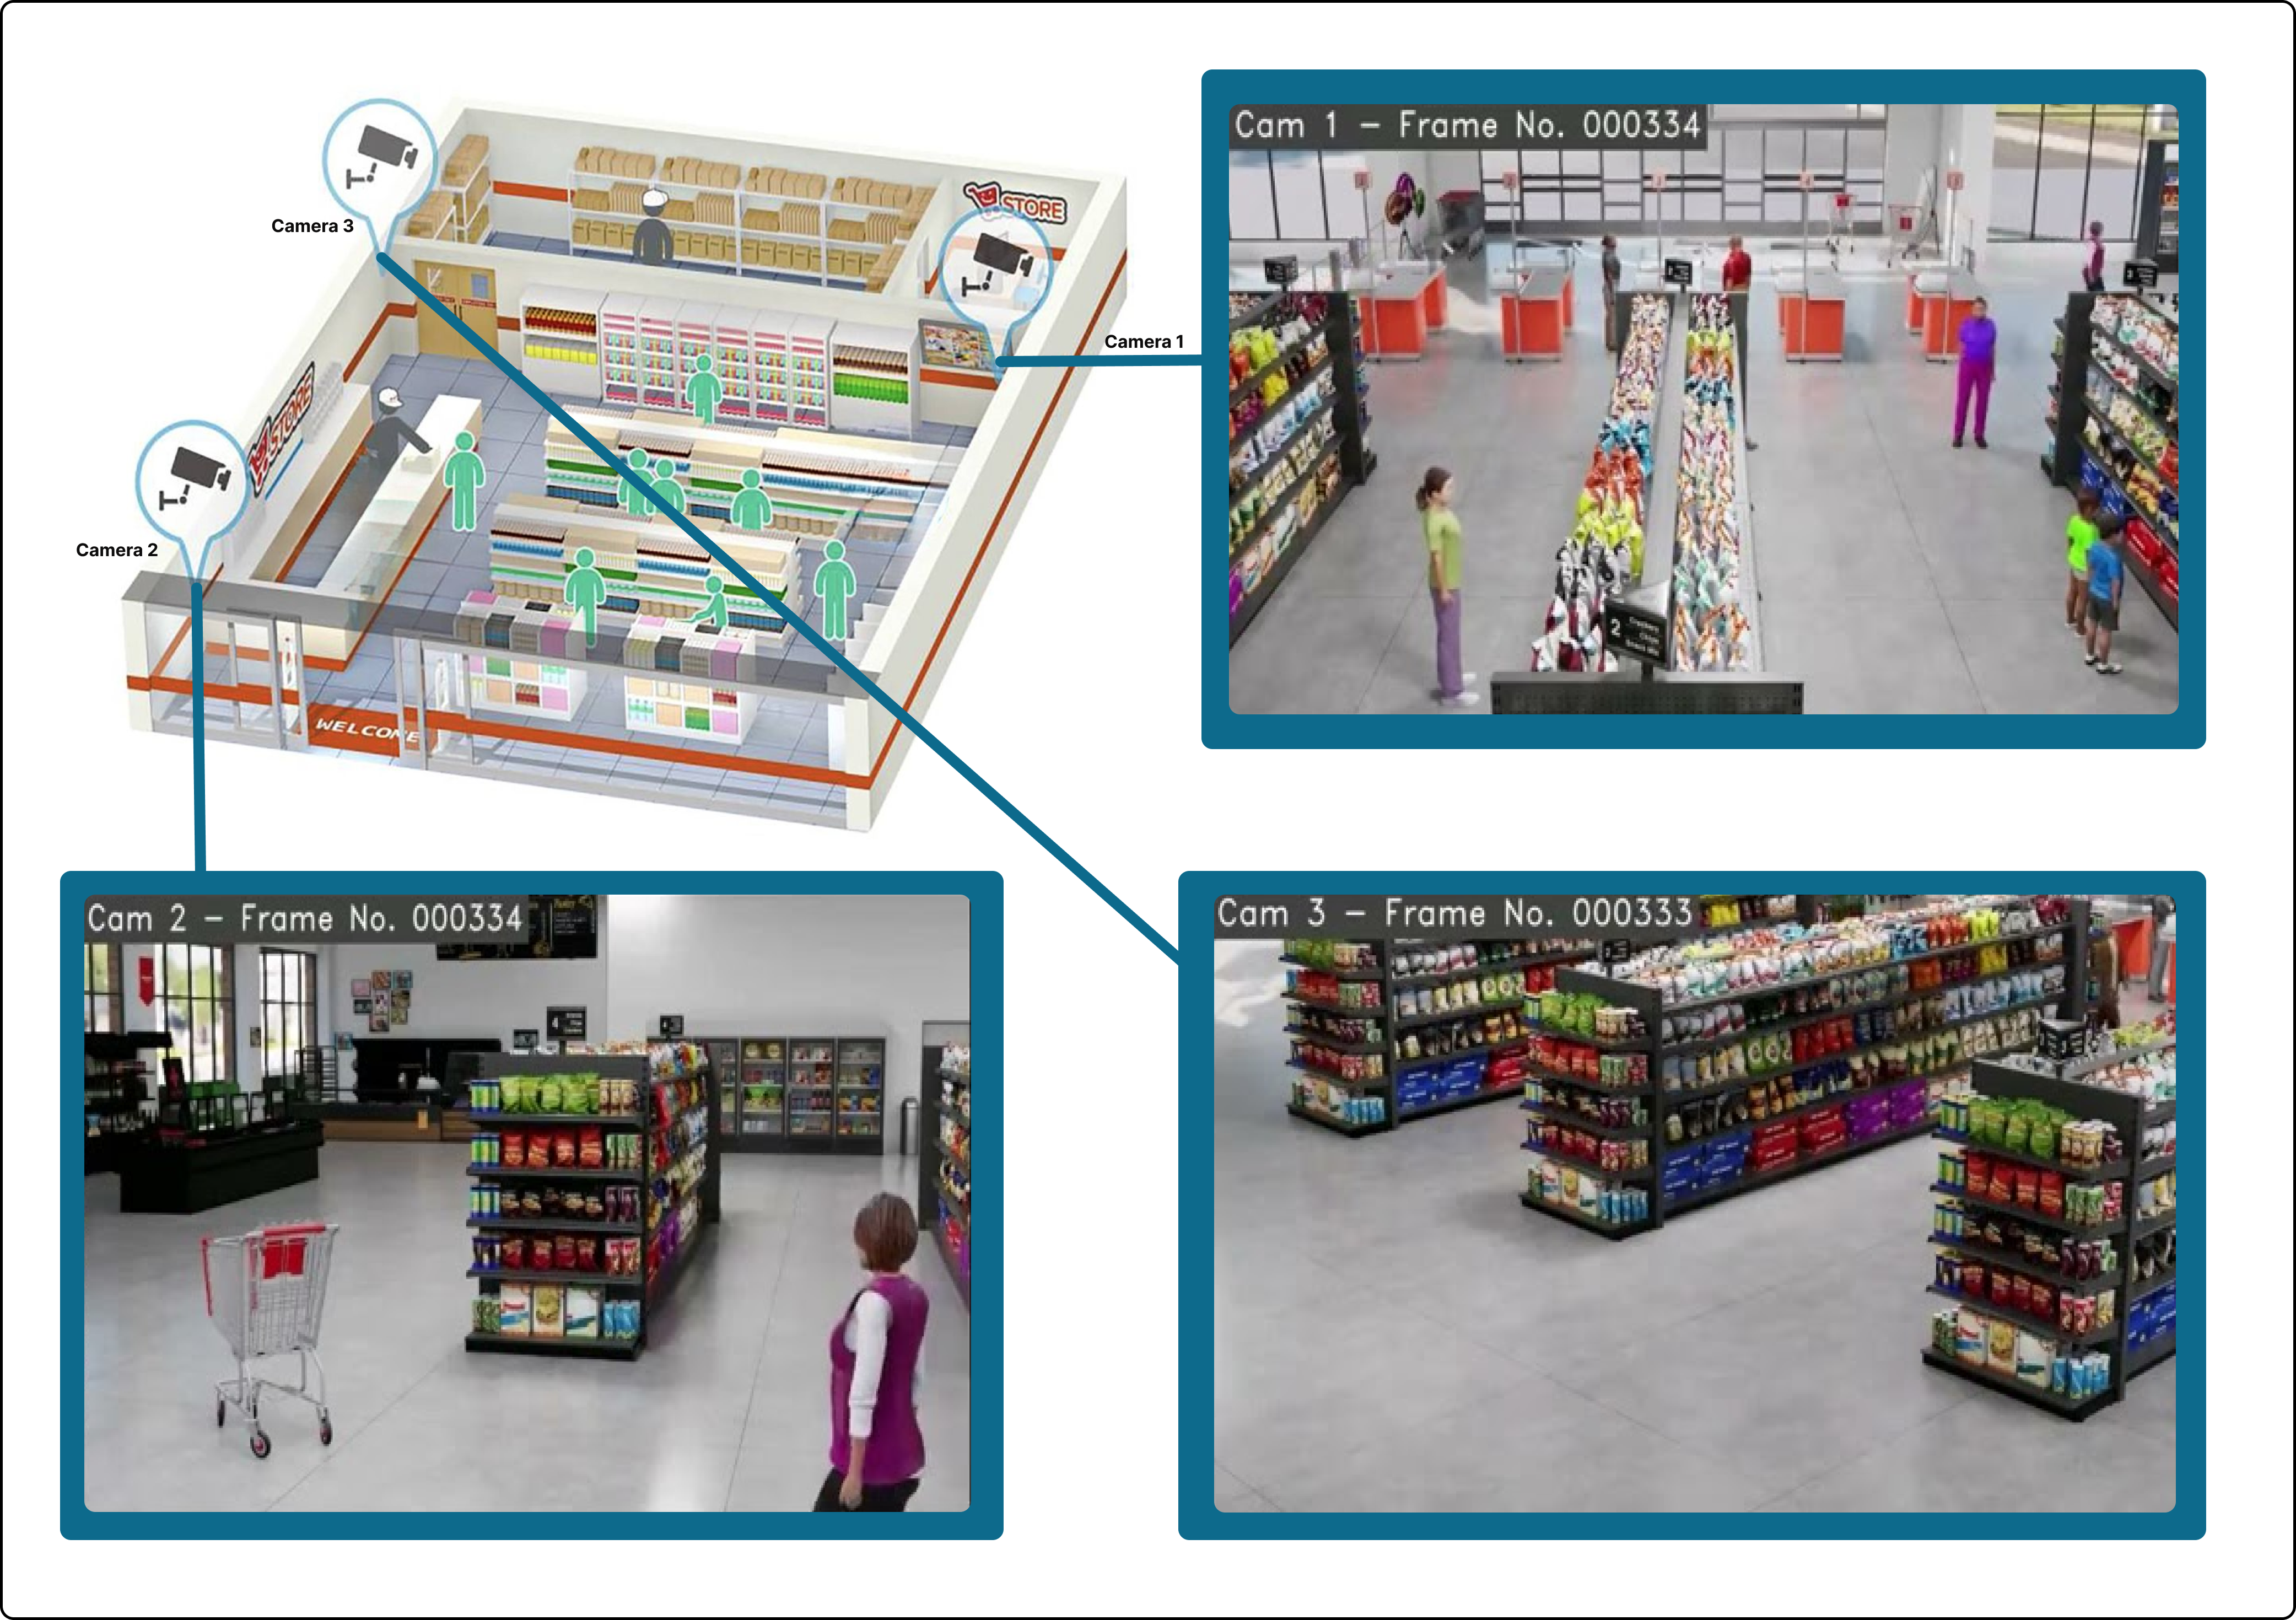
\includegraphics[width=1\linewidth]{fig/4.23}
	\label{fig:4.23}
\end{figure}

Furthermore, the recommendations were automatically produced based on the computed insights exemplified in Figure~\ref{fig:4.24}. These included:

\noindent - Leverage Top-Performing Aisles: Leverage the success of Aisle B, which accounted for 39.38\% of all foot traffic. Place new or high-margin products here to maximize visibility and drive sales.

\noindent - Replicate the Success of Long-Dwell Aisles: Study the characteristics of Aisle A, where customers spent an average of 1.44 minutes. Identify what makes this zone engaging, such as layout, product type, or sensory elements, and replicate it in other underperforming zones.

\noindent - Elevate Low-Performers Strategically: While overall performance is strong, consider improving the layout or visual appeal of less-visited aisles like Aisle E. This will balance store flow and reduce congestion in high-traffic zones.

\noindent - Continuous Monitoring: Establish a routine for weekly or monthly monitoring. Use these trends to make dynamic layout decisions and prepare promotions aligned with peak traffic patterns (e.g., around April 13, 2025).

The automated insight generation module of SUBAY successfully translated customer behavior metrics into scientifically derived and strategically valuable insights. Combining visualized data with coded logic referencing industry benchmarks empowered store managers to assess engagement performance quickly, identify top and underperforming zones, strategically place products, optimize layouts, and adapt marketing efforts to customer behavior. This section validated how SUBAY’s analytics engine supported evidence-based retail decision-making, providing data and interpretation tailored to business needs.

\begin{figure}[H]
	\caption[Sample Report’s Recommendations]{\newline \newline Sample Report’s Recommendations}
	\centering
	\includegraphics[width=0.75\linewidth]{fig/4.24.pdf}
	\label{fig:4.24}
\end{figure}

\section{Evaluate the Performance and Usability of the Multi-camera Object Detection System.}
This section outlines the results obtained from testing and evaluating the SUBAY system after its implementation. It includes the system's Zone-based Foot Traffic and Dwell Time Count results and the outcomes of functional and usability testing from the perspective of a retail store owner. These evaluations involved multiple testing phases, including system functionality checks, performance assessments, and end-user usability testing.

\subsection{Zone-based Foot Traffic and Dwell Time Count Results}

Video footage from four synchronized cameras was analyzed to evaluate the system’s capability in capturing zone-specific customer behavior. These cameras monitored six regions of interest (ROIs), labeled Zone A to Zone F. The system recorded key behavioral metrics for each zone, including Total Foot Traffic (number of unique customer entries), Total Dwell Time (measured in seconds and minutes), and Average Dwell Time per Customer, shown in Table 4.7. These metrics clearly show customer distribution and engagement within different store areas.

{
	\small
	\renewcommand{\arraystretch}{1.2}
	\begin{longtable}{|p{1.5cm}|p{1.5cm}|c|p{1.5cm}|p{1.5cm}|p{1.5cm}|p{1.5cm}|}
		\caption[Zone-based Foot Traffic and Dwell Time Count Results]{\newline \newline Zone-based Foot Traffic and Dwell Time Count Results} \label{tab:traffic_dwell} \\
		
		\hline
		\textbf{Zone Aisle} & \centering\textbf{Zone Labels} & \textbf{Total Foot Traffic} & \textbf{Total Dwell Time (s)} & \textbf{Total Dwell Time (min)} & \textbf{Average Dwell Time (s)} & \textbf{Average Dwell Time (min)} \\
		\hline
		\endfirsthead
		
		\multicolumn{7}{c}%
		{{\bfseries Table \thetable\ continued from previous page}} \\
		\hline
		\textbf{Zone Aisle} & \centering\textbf{Zone Labels} & \textbf{Total Foot Traffic} & \textbf{Total Dwell Time (s)} & \textbf{Total Dwell Time (min)} & \textbf{Average Dwell Time (s)} & \textbf{Average Dwell Time (min)} \\
		\hline
		\endhead
		
		\hline \multicolumn{7}{|r|}{{Continued on next page}} \\ \hline
		\endfoot
		
		\hline
		\endlastfoot
		
		Zone A & \centering Beauty Zone: Body and Bath Products & 73 & 6,322.58 & 105.38 & 86.61 & 1.44 \\
		\hline
		Zone B & \centering Beauty Zone: Face and Hair Care Products & 102 & 4,137.63 & 68.96 & 40.57 & 0.68 \\
		\hline
		Zone C & \centering Beauty Zone: Cosmetics & 46 & 5,899.81 & 98.33 & 128.26 & 2.14 \\
		\hline
		Zone D & \centering Assorted Home Essentials & 15 & 2,008.22 & 33.47 & 133.88 & 2.23 \\
		\hline
		Zone E & \centering Kitchen-\newline wares & 5 & 1,204.39 & 20.07 & 240.88 & 4.01 \\
		\hline
		Zone F & \centering Garden and Home Products & 18 & 783.96 & 13.07 & 43.55 & 0.73 \\
		\hline
		\textbf{Total} & & \textbf{259} & \textbf{20,356.59} & \textbf{339.28} & \textbf{1,032.76} & \textbf{17.21} \\
		
	\end{longtable}
}


The findings revealed notable behavioral trends. Zone B, the Beauty and Hair Care Products aisle, had the highest customer traffic, making it the most frequented area. Zone A, Body and Bath Products aisle, recorded the longest cumulative dwell time, identifying it as a high-engagement area with sustained customer attention. Zone D, Assorted Home Essentials, with low traffic, displayed an exceptionally high average dwell time, suggesting that visitors to this zone engaged more deeply or lingered longer, potentially due to product interest or browsing behavior. Zone E, Kitchenwares, exhibited minimal foot traffic but extended individual dwell durations, indicating a niche area of customer interaction.

These insights underscored the system’s ability to identify high-traffic zones for operational efficiency and high-dwell zones for strategic product placements. Retailers can use this data to optimize store layout, reallocate staff, and prioritize marketing efforts in zones with significant engagement potential.

\subsection{Functional and Usability Testing Results for Store Owner/\newline Manager at FashionLane Gift Shop}

Beyond system performance in customer tracking, it was equally important to assess how well the SUBAY system functioned in practice and how effectively end-users could interact with it. To this end, functional and usability testing was conducted with store owners and managers to evaluate the system’s responsiveness, ease of navigation, and overall user experience. Figure~\ref{fig:4.25} summarizes the functional testing results conducted with a retail store owner/manager (n=1). The evaluation focused on key functionalities of the SUBAY system, such as camera feed integration, customer detection and tracking, behavioral logging, dashboard analytics, access control, and system responsiveness.

\begin{figure}[H]
	\caption[Functional Test Result of Store Owner/Manager]{\newline \newline Functional Test Result of Store Owner/Manager}
	\centering
	\includegraphics[width=0.85\linewidth]{fig/4.25.pdf}
	\label{fig:4.25}
\end{figure}

All ten tested functions were marked as successful, achieving a 100\% success rate. These include consistent tracking across zones, detection of customer-shelf interaction, automatic behavior logging, and the correct data analytics presentation on the dashboard. Furthermore, the system ensured data privacy through secure admin access and did not collect personally identifiable information (PII). It also maintained performance stability even with simultaneous video streams. This indicates that the system was fully functional and operationally sound under real conditions.

Moving forward, the System Usability Scale (SUS) evaluation, shown in Figure~\ref{fig:4.26}, gathered the manager’s perceptions regarding ease of use. Using John Brooke’s methodology \citep{Carden2025}, each item was rated from 1 (Strongly Disagree) to 5 (Strongly Agree). The final SUS score was calculated by adjusting the scores of odd- and even-numbered questions accordingly, summing them, and multiplying by 2.5.

\begin{figure}[H]
	\caption[System Usability Scale (SUS) Result]{\newline \newline System Usability Scale (SUS) Result}
	\centering
	\includegraphics[width=0.85\linewidth]{fig/4.26.pdf}
	\label{fig:4.26}
\end{figure}

\noindent\textbf{Legend:}

\begin{tabular}{ll}
	\centering
	\textbf{Rating} & \textbf{Qualitative Description} \\
	SD & Strongly Disagree (1) \\
	D & Disagree (2) \\
	N & Neutral (3) \\
	A & Agree (4) \\
	SA & Strongly Agree (5) \\
\end{tabular}

\begin{table}[H]
	\centering
	\caption[System Usability Scale Final Result]{\newline \newline System Usability Scale Final Result}
	\label{tab:sus-result}
	\begin{tabular}{|c|c|c|c|}
		\hline
		\textbf{Average SUS Score} & \textbf{Grade} & \textbf{Adjectival Rating} & \textbf{Remarks} \\
		\hline
		87.5 & A+ & Best Imaginable & Acceptable \\
		\hline
	\end{tabular}
\end{table}

As shown in Table 4.8, the resulting SUS score was 87.5, corresponding to an A+ grade and an Adjectival Rating of “Best Imaginable.” This high score reflects excellent usability, indicating the user well-received the system in terms of design intuitiveness, feature integration, and confidence during usage. While the participant noted some concerns about complexity and the need for technical assistance, the overall experience was highly positive. These results validate that the SUBAY system is functionally reliable and user-friendly for retail owners or managers, ensuring its practical applicability in real-world retail environments.

}